\chapter{Monte Carlo Simulation}\label{chapt:MC}

To analyze the data from the large particle physics experiment, modeling of the events and the detector
plays an essential role. The processes of the $pp$ interaction and particle production are usually complicated
to resolve analytically. The same applies to the interactions within the detector volume. However, these 
tasks can be solved with the help of Monte Carlo (MC) simulation programs. These programs can be used to predict
the event yields and detector performance, to estimate the detector efficiencies, background processes rates etc.

In frames of this analysis it is needed to simulate the whole process of $pp \rightarrow t\bar{t} \rightarrow \bar{l}\nu bl\bar{\nu}\bar{b}$
in all the subprocesses (see Fig. \ref{fig:pp_all}). Therefor first the hard scattering tool has to be applied to simulate the collision and
production of the partons. The parton showering tools have to be applied to describe the electromagnetic and QCD
radiation of the final step particles. In the end of the process all the radiation finishes with forming the 
hadrons. There is also a possibility of interaction with the proton remnants. This interaction is described with
the underlying event process.

\begin{figure}[t]
  \centering
  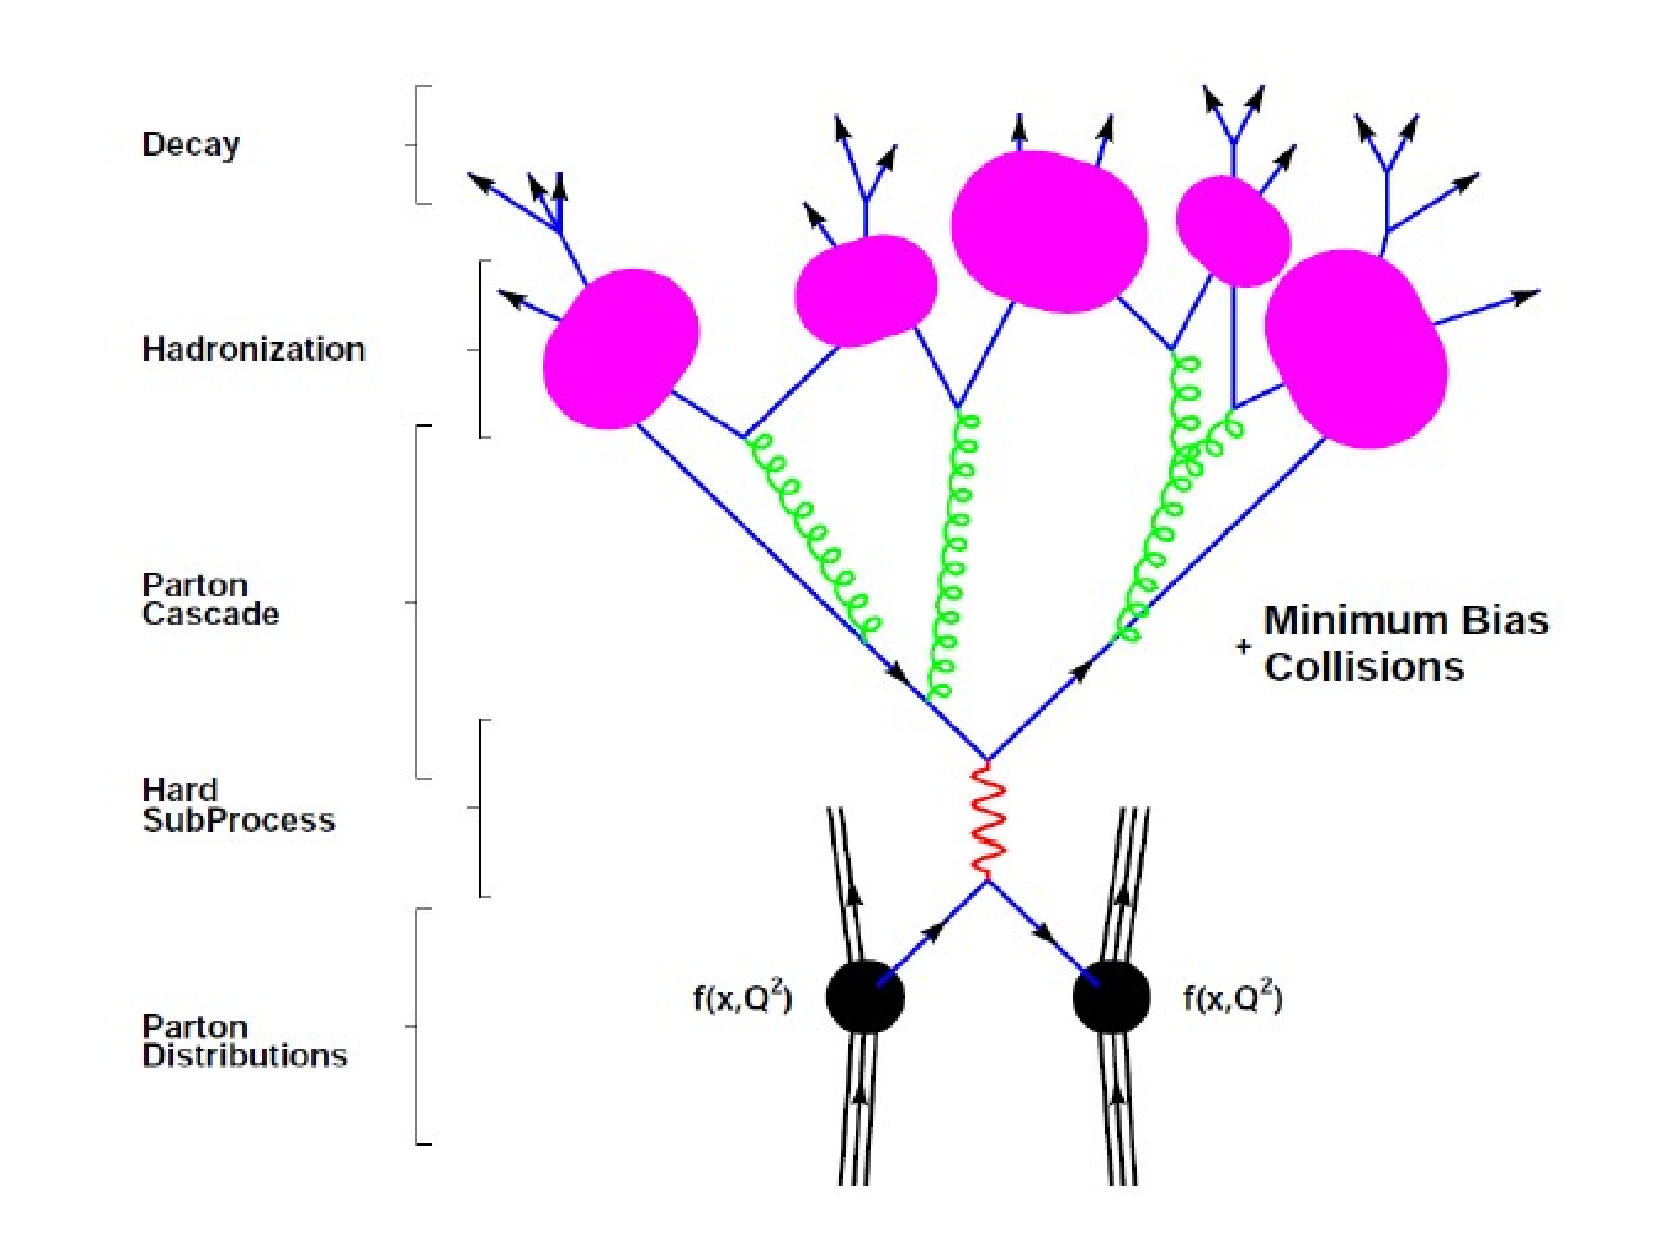
\includegraphics[width=0.8\textwidth]{03_simulation/plots/pp_all_proc.pdf}
  \caption{$pp$ collision scatch showing all the subprocesses.}
  \label{fig:pp_all}
\end{figure}

There are a number of general-purpose Monte Carlo (GPMC) generators (HERWIG \cite{Corcella:2000bw}, \PYTHIA6 \cite{Sjostrand:2006za}, SHERPA \cite{Gleisberg:2003xi})
on the market, which provide fully exclusive simulation of high-energy collisions. They consist of several components,
which describe the process starting from the very small distance scale up to the scale of hadrons and their decays. 

To finalize the analysis modeling, after simulating the particle production and decay processes, it is necessary 
to push the products of these simulation through a model-detector. The model-detector simulated all the particles 
interaction with matter and possible noises. Such a detector model can be used also to predict the performance 
of the future facilities.

This chapter gives a brief overview of the processes which were simulated for this analysis, and tools used for 
the simulation.

\section{Different Monte Carlo Models and Generators}

This section gives an overview of models used in the MC generators for the simulation. The MC generators used
for this analysis are listed and briefly described.

\subsection{Hard Scattering Models}

The \textit{hard scattering} describes the interaction of partons, which emerged out of the proton (in the case of 
this analysis - two gluons or quark-antiquark pair) and take part in the production process which is being studied.

The parton interaction is taking place in the high energy regime, so that $\alpha_{s} \ll 1$ (see sec. \ref{sec:strong_int}). 
This allows the perturbative calculations of the process -- expansion the equations according to the order of $\alpha_{s}$.
Thus, the processes of hard interaction may be calculated in different orders of $\alpha_{s}$: the higher the order accepted
for the calculations, the more precise the calculation should be. However, there are many subtleties with calculating the 
higher orders, that is why the MC generators are usually limited to LO or NLO calculations.

The initial momenta of partons are to be chosen taking to account the PDFs.

\subsection{Parton Showering}

The hard scattering models are fixed to some order of perturbative calculations. This is not sufficient to describe the 
whole picture of the event. That is why the special \textit{parton showering} techniques were developed to simulate the 
higher order effects. It describes the irradiation of the colored objects in the initial (partons) and final state,
following the momentum transfer from the higher interaction scales down to the lowest scales of confinement (hadronization) --
to the order of 1 GeV.

Parton showering describes two kinds of irradiation: \textit{initial state radiation}, or the irradiation of colored partons
before they enter the hard interaction, and the \textit{final state radiation}, or the irradiation of inside or at the final
state of the hard scattering.

\begin{itemize}
 \item \textbf{The final state radiation} is described by sequential splitting of the colored objects with energy lessening
 after each splitting. This process is repeated until some evolution criterion is reached. Such criteria may be connected
 with the energy fraction of irradiated object or with the opening angle between the parent and emitted colored object.
 
 \item \textbf{The initial state radiation} is produced in the similar way to the final state radiation, but inverting
 the process such that the colored objects out of the shower collapse back to the initial partons out of the protons.
\end{itemize}

Now if the parton shower is simply added to the hard scattering, the same process can be modeled twice. Some radiation
may be already taken to account in the hard interaction but it is still produced in the parton showering. This means 
there has to be a way to allow only one mechanism to produce this process.

\subsection{Hadronization Models}

In context of the MC generators, the \textit{hadronization} is the process by which a set of colored objects (after showering)
is transformed into color-singlet particles, hadrons, which can further decay into another hadrons. This transition is non-perturbative
with the scale $Q_{had}$ (with $\alpha_{s} \sim 1$), which is identical to she shower energy limit. Thus, the full QCD calculations
are not possible. The hadronization scale may be defined slightly different in different generators.

The main difference between the MC hadronization model and fragmentation function description of hadronization in QCD, is that former
is defined only at the hadronization scale, while the letter is defined at any scale.

There are two models which may be the basis for the MC generator hadronization:

\begin{itemize}
 \item \textbf{String model}. The basics for this model were taken from the string model of elementary particle physics \cite{Artru:1974hr}.
 the main feature being exploited is that the so called \textit{linear confinement}, or that the potential of the color dipole 
 between the color and anticolor is growing with separation of the charges on the distances of about a femtometer.
 
 One of the most popular generator string models is the \textit{Lund model}. The linear color potential between the quarks is 
 expressed as $V(r) = \kappa r$, which can be described as a string with tension $\kappa \sim 1\,GeV/fm \sim 0.2\,GeV^{2}$. 
 The Coulomb interaction is neglected in the Lund model. The physical picture of this potential is the colored tube between quark
 and antiquark. As the quarks start to separate in space, the string grows and finally breaks via the process of a new quark-antiquark
 pair creation, $(q\bar{q}) \rightarrow (q\bar{q}') + (q')\bar{q}$. The illustration of this process is shown in Fig. \ref{fig:Lund}.
 
 \begin{figure}[h]
  \centering
  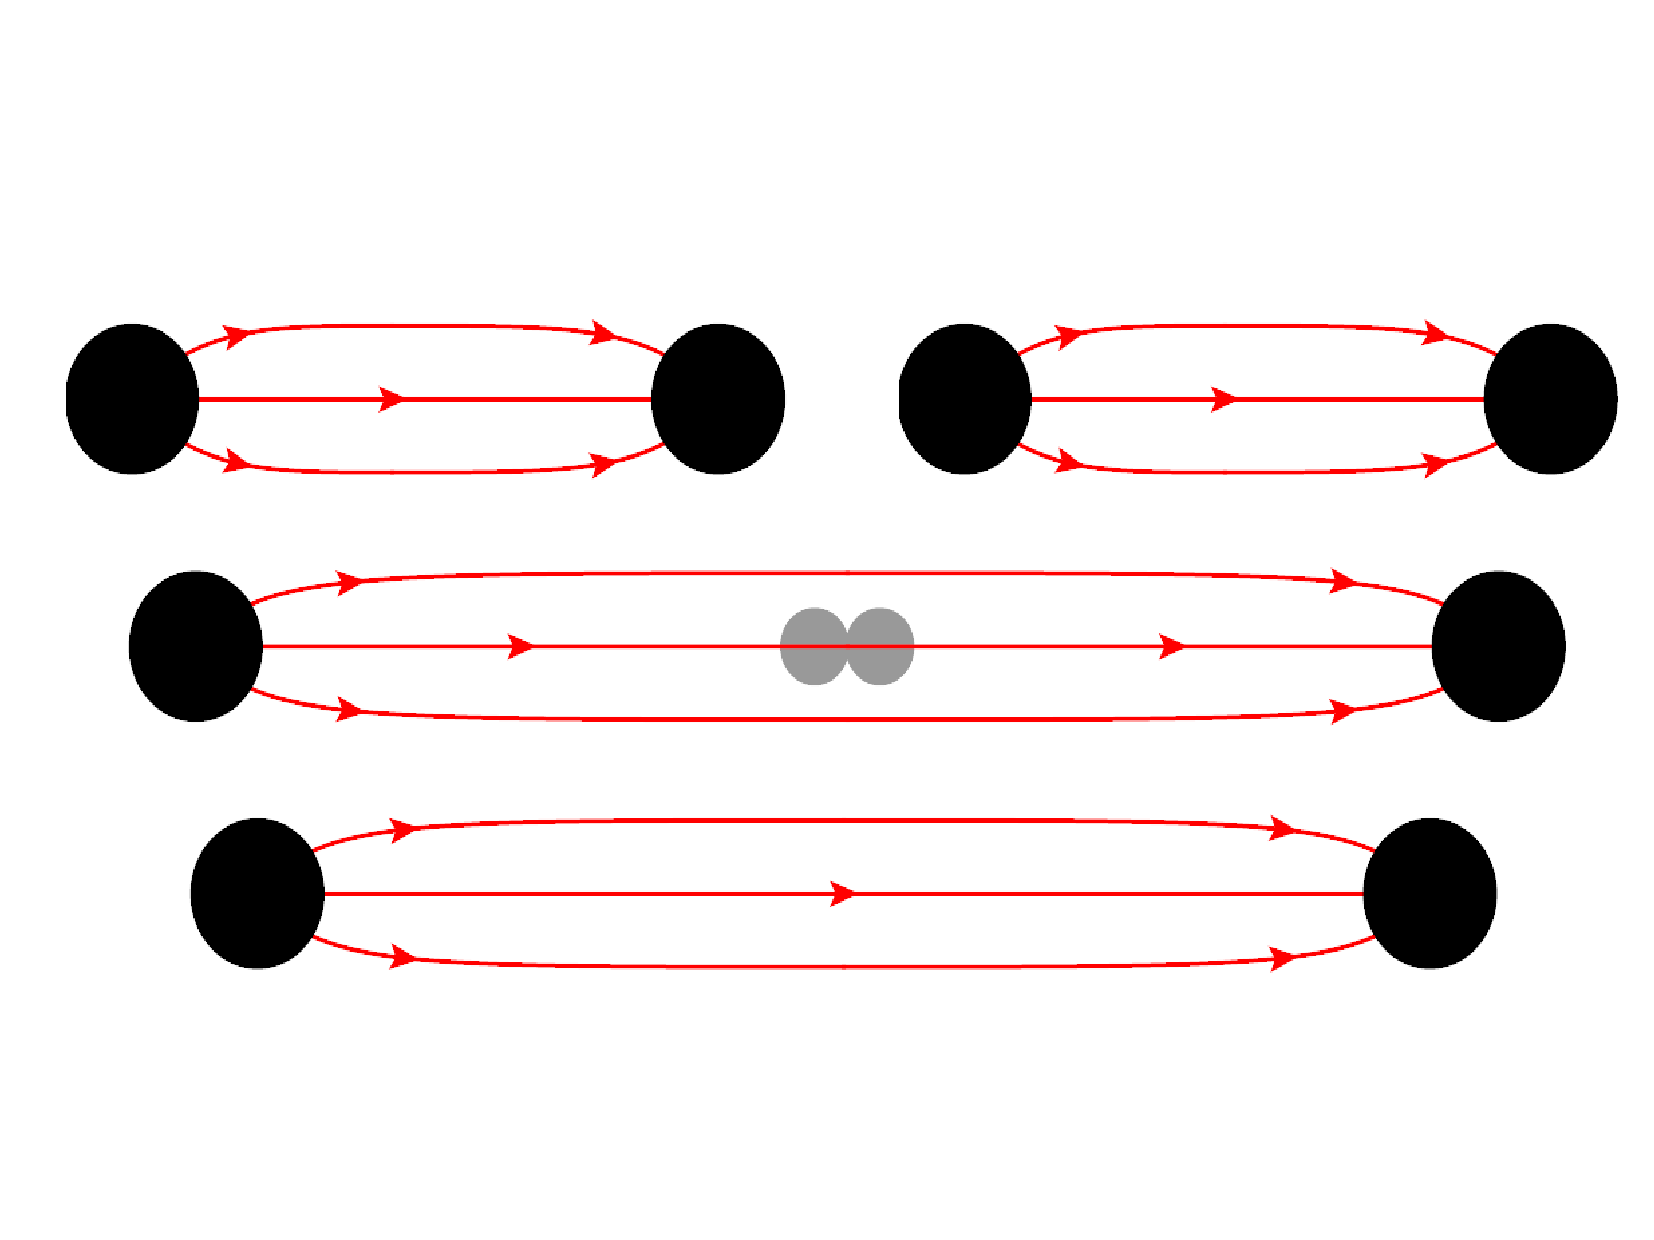
\includegraphics[width=0.8\textwidth]{03_simulation/plots/Lund_hadr.pdf}
  \caption{Illustration of string breaking by quark pair-creation in the string field. Black spots are the quarks and the red
  stripes are the field illustration.}
  \label{fig:Lund}
 \end{figure}
 
 The gluons are represented with the transverse kinks in the strings. They have to be connected to the field strings from both
 sides, while quarks have the connection only from one side.
 
 The mechanism described above is producing mesons, as the states with two quarks are formed. The baryons can be also produced
 in Lund model, but in the process where the string breaking produces the pair of diquarks.
 
 The hadronization stops after reaching the point when there is not enough energy to create a hadron.
 
 \item \textbf{Cluster model}. This hadronization model is based on the \textit{preconfinement} \cite{Amati:1979fg}, or the
 observation that the color-singlet parton subsystems, called \textit{clusters}, occur with the universal mass distribution
 depending only on the scale $Q_{0}$ at which they were formed, and not on the starting scale of the showering.
 
 The other key idea of the model is that the gluons are forced to split into quark-antiquark pair at the end of the parton shower.
 The clusters formed by the gluon splitting are then forced to decay into the on-shell hadrons.
 
\end{itemize}

\subsection{Hadron Decay}

The hadrons formed after hadronization, are so-called primary hadrons. They can be unstable, thus they decay into secondary hadrons
until the set of stable particles\footnote{A typical definition of stable particles in hadron colliders is that their
lifetime, $c\tau$, is greater than 10$mm$. This includes the weakly decaying strange baryons.} is formed.

One would expect, that all the needed information for the decay would be present in the Particle Data Group (PDG) listings \cite{PDG-2012}.
However, this information is often not unique and requires multiple choices to be made. The more hadrons are included into the simulation,
the more choices one has to make.

The individual properties of each generator are:

\begin{itemize}
 \item which hadrons to include into simulation;
 \item which decay modes to allow;
\end{itemize}

In general, the simulation of hadron decays is based on a combination of experimentally measured properties and theoretical assumptions, which
might also differ from generator to generator.

\subsection{Underlying Event}

The \textit{underlying event} (UE), in terms of the MC generators, is the activity beyond the basic process, like multiple parton-parton interactions
(MPI) between the beam particles. The MPI may sometimes give a rise to two or more back-to-back jets (if there were more hard parton-parton interactions
in one proton-proton collision). This case is, however, very rare. The main impact is coming from the soft MPI. They may affect, for example, the 
missing $E_{T}$ distribution or increase the activity in forward direction (break-up of the beam remnants).

The first and the basic Monte Carlo model for the UE is given in \cite{PhysRevD.36.2019}. There are some basic assumptions involved into
this model, like, for example, the interactions can't use more momentum than it is available in the parent hadron (proton in case of this analysis).

The UE models are usually tuned to the experimental conditions and on experimental data. The model derived on the CMS data collected at $\sqrt{s} = 0.9\, TeV$
and $\sqrt{s} = 8\,TeV$ is called the $Z2*$ model \cite{Chatrchyan:2011id}.


\subsection{Monte Carlo Generators}

After describing the main principles behind the MC simulation of the events for the experiments in the field of elementary particle
physics, the list of the generators used for this analysis will be given.

\subsubsection{$\PYTHIA$ 6}

\PYTHIA \cite{Sjostrand:2006za} is the general-purpose event generator. It is set to describe the collisions between hadrons
or the same generation leptons. \PYTHIA includes more than 200 hardcoded
hard subprocesses, which include the Standard Model events but also some exotic and beyond Standard Model processes \cite{Buckley:2011ms}.

For this analysis \PYTHIA is used with the LO QCD accuracy.

For the parton showering, the kinematic limit is set on the transverse momentum related variables.

For the hadronization, the Lund string model is used.

The $Z2*$ model for the UE simulation is conventionally used in \PYTHIA for the UE simulation.

\subsubsection{$\HERWIG$}

\HERWIG \cite{Corcella:2000bw} is a general-purpose generator as \PYTHIA. It can model hadron-hadron, lepton-lepton and hadron-lepron collisions.

\HERWIG is able to produce a fairly large variety Standard Model QCD and electroweak processes and elementary subprocesses beyond the standard model.
For this analysis this generator is used with the LO precision.

The parton showering is limited by the scale $Q^{2} \sim 1 - cos\theta$, where $\theta$ is an angle between the parent and emitted partons.

The cluster model is used for the hadronization in \HERWIG.

The model for the UE used by \HERWIG was originally derived by ATLAS and is called AUET2 \cite{ATL-PHYS-PUB-2011-009}.

\subsubsection{MadGraph}

Unlike \PYTHIA and \HERWIG, \MG is not a general-purpose generator. It is used to generate the hadron-hadron $pp$ and $p\bar{p}$ collisions.
It gives the LO precision outcome for the hard processes with maximum 8 particles in the final state. 

\MG is a matrix element generator. It doesn't include hadronization and provides only leptons, quarks and gluons as the result. These outcome
is afterwards interfaced to some general-purpose generator to generate the rest of the information. The combination \MG+\PYTHIA provides a better
results compared to \PYTHIA only, as the \MG hard interaction is more specifically tuned for the needs of hadron-hadron collisions. 

The problem of double counting of objects in showering, while interfacing \MG to the general-purpose generator, is solved with the help of the 
MLM scheme \cite{Mrenna:2003if}.

\subsubsection{Powheg}

The \Powheg (Positive Weight Hardest Emission Generator) event generator \cite{Frixione:2007vw} provides the modeling of the hard interaction 
with the NLO accuracy. The \Powheg method doesn't have parton showering included. Thus, it has to be also interfaced with \PYTHIA or
\HERWIG for a full event description.

\subsection{MC@NLO}

The \MCNLO \cite{Frixione:2002ik} is also an event generator which generates the hard emission with the NLO precision. For the showering
it has to be interfaced with general-purpose generators, as it is also done for \Powheg. 

\MCNLO is designed for hadron collisions being able to produce top quark pairs, Higgs boson, vector boson (single or in pairs), single top,
lepton pairs and associated $H+W/Z$.

\MCNLO generator provides some events with negative weights. However, the fraction of these events is very small \cite{Frixione:2002ik}.


\section{Detector simulation}

After the bare event with all the particles was simulated, it can be pushed through a detector simulation. That means that all of the particles 
will interact with the material and fields of the model of a real detector. This allows the close to experimental measurements, estimation of the 
detector efficiencies and performance, prediction of the performance and comparison of the theoretical models encoded in the event generators to
the experimental measurements. The simulation of the detector is performed by means of the Geant simulation toolkit.

\subsubsection{Geant 4}

Geant4 (GEometry ANd Tracking) \cite{Agostinelli:2002hh} is a toolkit designed for an accurate simulation of passage of particles through matter.
The tool includes all the aspects of the simulation, like geometry of the system, the materials involved, fundamental particles of interest,
tracking of particles through materials and electromagnetic fields, the physics processes governing the particle interactions, the response of
sensitive detector components, the storage of events and tracks, the vizualization of detector and particle trajectories and the analysis of
the data on different levels of details.

Geant can handle the particle interactions on a very wide energy scale. It also includes a large amount of known particle interaction models
from all over the world.

For the needs of the CMS experiment it was also tuned to correct the deviations between the experimental data and simulation.

An example of the display of fully simulated event is shown in Fig. \ref{fig:Evt_display}.

 \begin{figure}[h]
  \centering
  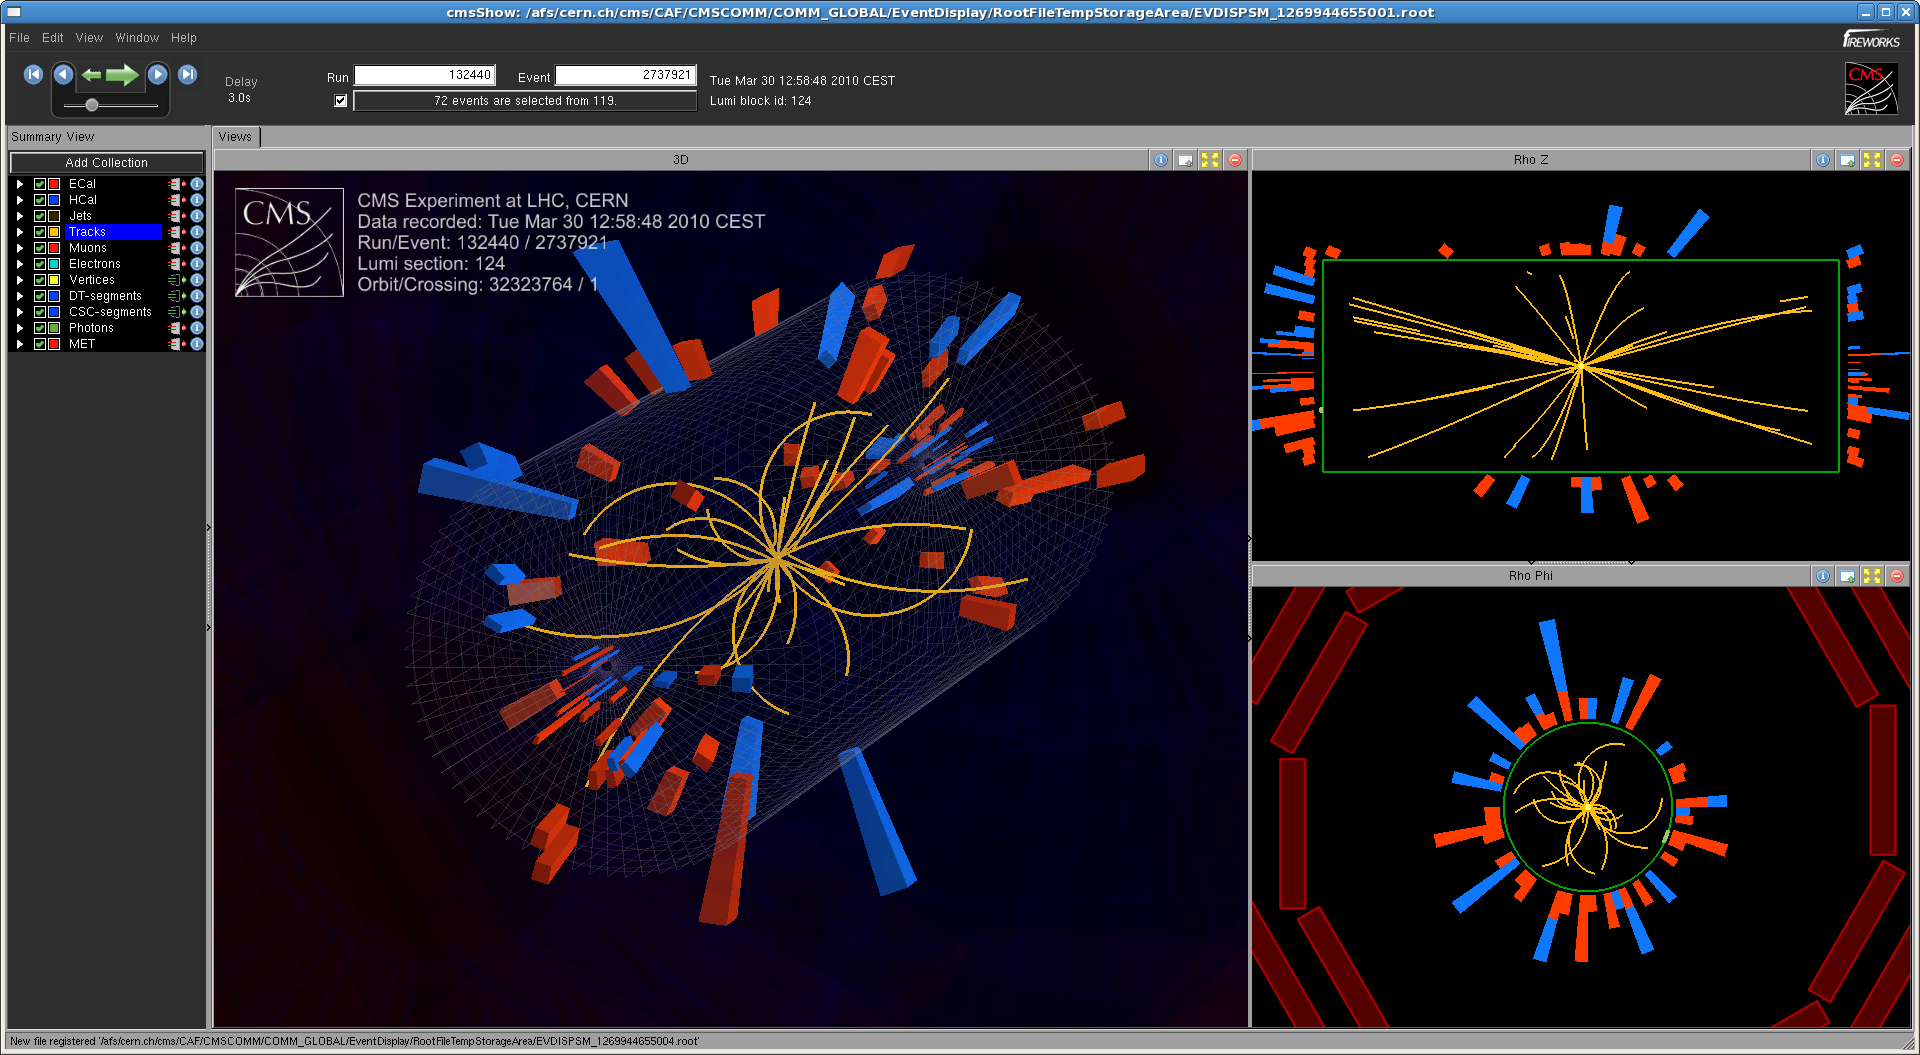
\includegraphics[width=1.0\textwidth]{03_simulation/plots/CMS1stEvent.png}
  \caption{Display of the simulated event in the CMS detector model.}
  \label{fig:Lund}
 \end{figure}